\chapter{Psalm 76}

\begin{figure}
  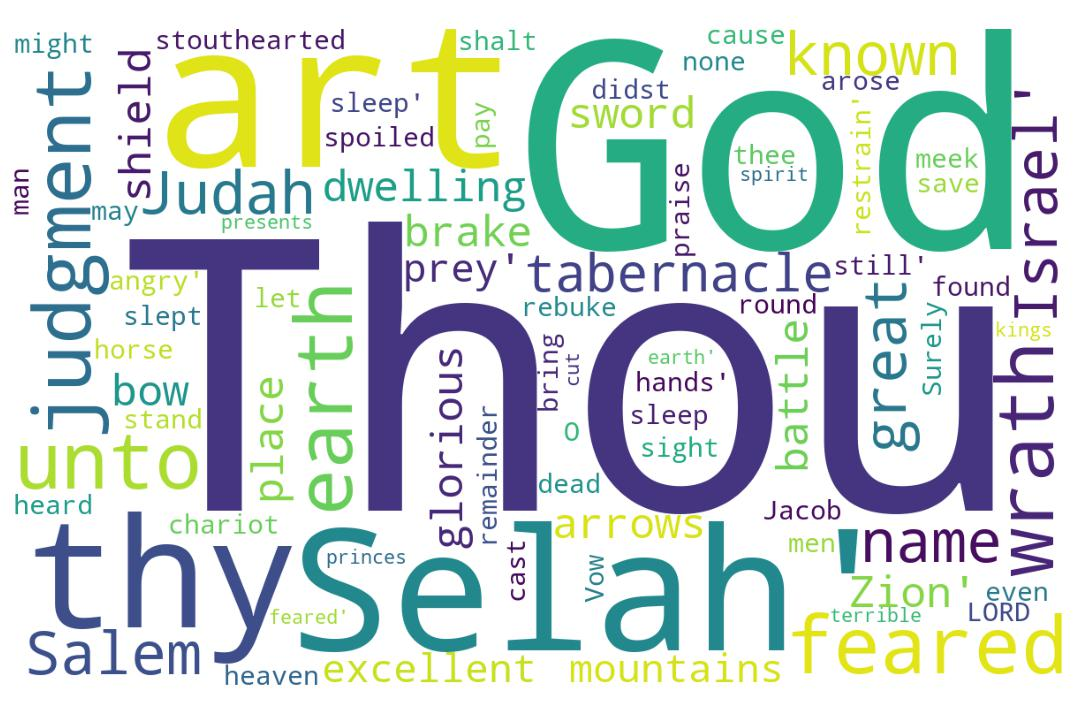
\includegraphics[width=\linewidth]{19OT-Psalms/Psalm76-WordCloud.jpg}
  \caption{Psalm 76 Word Cloud}
  \label{fig:Psalm 76 word Cloud}
\end{figure}

\marginpar{\scriptsize \centering \fcolorbox{bone}{lime}{\textbf{TWO KINDS OF PEOPLE}}\\ (Psalm 76:1-12) \begin{compactenum}[I.][8]
     \item Those \textbf{Shielded} \index[scripture]{Psalms!Psa 076:03}(Psa 76:3)
    \item Those \textbf{Spoiled} \index[scripture]{Psalms!Psa 076:05}(Psa 76:5)
    \item Those \textbf{Put to Sleep} \index[scripture]{Psalms!Psa 076:06}(Psa 76:6)
    \item Those \textbf{Seen} \index[scripture]{Psalms!Psa 076:07}(Psa 76:7)
    \item Those \textbf{Stilled} \index[scripture]{Psalms!Psa 076:08}(Psa 76:8)
    \item Those \textbf{Subdued} \index[scripture]{Psalms!Psa 076:08}(Psa 76:8)
    \item Those \textbf{Saved} \index[scripture]{Psalms!Psa 076:09}(Psa 76:9)
\end{compactenum}}
    




% \textcolor[cmyk]{0.99998,1,0,0}{
\footnote{\textcolor[rgb]{0.00,0.25,0.00}{\hyperlink{TOC}{Return to end of Table of Contents.}}}\footnote{\href{https://audiobible.com/bible/psalms_76.html}{\textcolor[cmyk]{0.99998,1,0,0}{Psalm 76 Audio}}}\textcolor[cmyk]{0.99998,1,0,0}{To the chief Musician on Neginoth, A Psalm \emph{or} Song of Asaph.}\\
\\
\textcolor[cmyk]{0.99998,1,0,0}{In Judah \emph{is} God known: his name \emph{is} great in Israel.} %\footnote{[RUCKMAN] The Psalm is on the Second Advent. God is not known in Judah now, nor has His ``name'' been ``great in Israel'' for 1,950 years. The name “Jehovah” may be great in Israel now, but if we are to believe Deuteronomy 32:15--22; Mark 7:3--13; and Romans 10:1--3, the name is only lip service. God is NOT known, and will not be “known in Judah and Israel” until Hebrews 8:8--12. In this age, God is known, and His “name is great,” among the Gentiles (Acts 28:28), but only because of the Jew (“Judah”). The term “Jew” was given to Judean Jews in Jerusalem (John 5:16, 18), and inspite of tons of anti-Semitic hogwash about “Khazars,” “Edomite usurpers,” and the “ten lost tribes,” salvation is still of the “Jews,” and I don’t mean “Israel” or “the Israel of God” or the “house of Israel.” I mean “Jews,” as in Judean Jews from Judah (vs. 1).\cite{Ruckman1992Psalms}}
[2] \textcolor[cmyk]{0.99998,1,0,0}{In Salem also is his tabernacle, and his dwelling place in Zion.} %\footnote{[RUCKMAN] ``In Salem.” The word is kin to “Shalom” and “Shiloh,” meaning “peace.” God’s dwelling place in this age is NOT in Zion, and He has no tabernacle there; Asaph is prophesying (see the introductory notes). Those who tried to historicize verse 2, and lay it on David or Solomon, have two problems. In the first place, wars do NOT stop in David’s time, nor do they stop in Solomon’s time. The breaking up of weapons in verse 3 is punctuated by our good, old friend “Selah,” showing anyone but a Bible-correcting Hebrew scholar that we are to look at Haggai 2:9 and Zechariah 14 for the meaning of the verse. The word Jerusalem means “city of peace,” so:\cite{Ruckman1992Psalms}
%\begin{compactenum}
%\item It is captured by the Jews in Judges 1:8, but they have to fight against it again to retake it in 2 Samuel 5:6–10. 
%\item Shishak attacks it in 2 Chronicles 12:9.
%\item Jehoash goes after it in 2 Kings 14:13, Rezin in 2 Kings 16:5, and Sennacherib in Isaiah 36 and 37.
%\end{compactenum} 
%Nebuchadnezzar goes up to it three times; Ptolemy Soter attacks it in 320 B.C., Antiochus defiles it in 203 B.C., Scopus attacks it in 199 B.C., and Antiochus hits it again in 168 B.C., and then again “for good measure” in 162 B.C. “City of Peace.” Fantastic, isn’t it? Imagine the commentators thinking that God stopped all the wars with the destruction of David’s foes or Solomon’s or even Hezekiah’s foes (Sennacherib)! Kroll is as tongue tied when he stares at the passage as a calf looking at a “new gate.” He doesn’t know what on earth to do with it. Hyracannus attacks Jerusalem in 65 B.C. Pompey follows suit in 63 B. C. Herod does a bang up job in 39 B.C., and then Titus finishes it off in A.D. 70. But the best is yet to come. Chosroes the Persian attacks it in A.D. 559 after the Romans did it in A.D. 135. Then Afdal takes it in A.D. 1098, after Omar destroyed it in A.D. 637. Then the Crusaders take it (A.D. 1099) only to lose it to Saladin (A.D. 1187). Never fear. Allenby “liberated” it in A.D. 1917, and then the Arabs took over fighting against it with Lebanese, Egyptians, the PLO, the Pope, and the American news media to help them out.\cite{Ruckman1992Psalms}}
[3] \textcolor[cmyk]{0.99998,1,0,0}{There brake he the arrows of the bow, the \fcolorbox{bone}{lime}{shield}, and the sword, and the battle. Selah.}
[4] \textcolor[cmyk]{0.99998,1,0,0}{Thou \emph{art} more glorious \emph{and} excellent than the mountains of prey.} %\footnote{[RUCKMAN] The “thou” is Mt. Zion (see Ps. 68:15 and comments). Two thoughts are present. Mountains which have wild animals on them who take “prey” (Song of Sol. 4:8), are not to be compared with a mountain like Mt. Zion, which not only had the temple on the place where God ordained sacrifices to be made, but also was the location of the Ark of the Covenant which held the Book (Deut. 31:26). The “oracle” of God (1 Kings 6:5) was located on Mt. Zion. The second thought is that the earthly powers represented by mountains (see Rev. 17, for example, and Jeremiah 51:25) are no equal for the “mountain of the Lord” (see Isa. 2:2). He is “king of the mountain,” and His “mountain” will tower above McKinley, Blanc, Whitney, Ararat, Everest, etc., for its prototype (see Heb. 12:22) is already a good bit higher than the entire Milky Way.\cite{Ruckman1992Psalms}}
[5] \textcolor[cmyk]{0.99998,1,0,0}{The stouthearted are \fcolorbox{bone}{lime}{spoiled}, they have slept their sleep: and none of the men of might have found their hands.} %\footnote{[RUCKMAN] Literally, in the sense of Saul (1 Sam. 26:12), who is a type of the Antichrist; doctrinally, in the sense of being dead (see Isa. 26:14; Dan. 12:2). Several things happen at Armageddon that the prophetic expositors never picked up. One of them is that the Antichrist’s troops will kill each other (Judg. 7:22), their flesh will rot on their faces (Zech. 14:12), and their horses will go blind and rabid in the midst of the attack (Zech. 12:4). These are the UN troops (Rev. 19:19) who hope to overthrow the rider on the “white horse” (Rev. 19:10-–14). Observe the advanced revelation found in the AV text which all of the commentators (naturally) missed. When Kroll sees that the “chariot” goes into a dead sleep, as well as the “horses” he mumbles, “the cavalries of the oppressors were stopped.” (Yeah, sonny, they sure were.) The New Idiotic Version (NIV) can’t handle it, so they say that “they lie still.” The Living Baboon says “fell.” The RSV, NRSV, NNRSV (and NNNRSV) take the word “chariot” clean out of the text so they don’t have to deal with the problem: “Both rider and horse lay stunned.” Typical. Absolutely typical of the brand of scholarship you would get at Bob Jones or Liberty University. \cite{Ruckman1992Psalms}}
[6] \textcolor[cmyk]{0.99998,1,0,0}{At thy rebuke, O God of Jacob, both the chariot and horse are cast into a \fcolorbox{bone}{lime}{dead sleep}.} %\footnote{[RUCKMAN] But after 1910, the “chariot” could go to “sleep.” What auto mechanic doesn’t know that? As a matter of fact, the motor can even “die,” and what driver didn’t know that? If it is “awake” but not moving, it is “idling,” and who didn’t know that but the commentators who couldn’t imagine chariots going to sleep? They went to sleep on the Russian front (1942--1944) because the tank fluids froze, or the rats shortcircuited the controls by chewing through the insulation. In my generation (1921--1949), we called automobiles by a peculiar name; we called them “chariots.” A chariot can “malfunction.”\cite{Ruckman1992Psalms}}
[7] \textcolor[cmyk]{0.99998,1,0,0}{Thou, \emph{even} thou, \emph{art} to be feared: and who may stand \fcolorbox{bone}{lime}{in thy sight} when once thou art angry?}
[8] \textcolor[cmyk]{0.99998,1,0,0}{Thou didst cause judgment to be heard from heaven; the earth feared, and was \fcolorbox{bone}{lime}{still}.}
[9] \textcolor[cmyk]{0.99998,1,0,0}{When God arose to judgment, to \fcolorbox{bone}{lime}{save} all the meek of the earth. \fcolorbox{bone}{red}{\textcolor{white}{Selah}}.} %\footnote{[RUCKMAN] All is clear. God “arises” in verse 9 (see Ps. 3:7, 7:6, and 9:19), and not one time is this a reference to God helping anyone out between 500 B. C. and A.D. 2002. “Selah” comes to our aid again to give us the key for judging the critics of the Book. It is a “handy reference” to use in throwing out 80 percent of the rubbish on the Psalms published by Zondervan, Baker, Eerdmans, and Bob Jones University Press. Verse 11 is the exact match for the comments under Psalm 68:29--32, which see. The “vow” of verse 11 is the exact millennial match to Psalm 65:1 and Psalm 50:14, which see. Verse 12 is Armageddon fulfilled, as in Psalm 2:2, 89:27, and Isaiah 24:21. This is a literal destruction at the Advent. In verse 8, we learn that the earth has more sense than most of its inhabitants. The judgment is “heard from heaven,” literally, in Hebrews 12:25; Haggai 2:6; and Psalm 50:3--5 (which see). All of the commentators miss all the references. (This is just as natural for them as breathing.) Note “the meek” of the Sermon on the Mount (Matt. 5:5), showing up in verse 9. \cite{Ruckman1992Psalms}}
[10] \textcolor[cmyk]{0.99998,1,0,0}{Surely the wrath of man shall praise thee: the remainder of wrath shalt thou restrain.} %\footnote{[RUCKMAN ]The destructive critics of the AV come apart at verse 10, which stands in the AV as clear as crystal. The idea is that man’s hatred against God and God’s people will be turned backwards, so that instead of destroying God’s people or stopping God’s hand, God “banks it off the siderail”—He winds up getting glory from it (see Exod. 14:4; Rom. 11:30–34; and Exod. 9:16, 18:11). “The remainder” is a reference to any wrath that does not produce praise for God or glory to Him. Cases are too numerous to mention, the main ones being men killing each other over religious and political issues to the tune of 80,000,000 casualties since A.D. 70. Individual murders (five a day in Detroit, one a day in Las Vegas, two a day in Miami, and ten a day in Washington, D.C.) do not praise God, but murderers are restrained so that total mayhem and murder don’t break out internationally with five hundred killed daily in Memphis, Atlanta, London, Paris, New York, Rome, Madrid, Tokyo, Bombay, Athens, Oslo, Seattle, and Oklahoma City. What wrath does not praise God is held in check so it doesn’t annihilate mankind altogether. Today the Arabs are restrained by “the restrainer” (2 Thess. 2:6–7); otherwise, they would have pushed Israel off into the Mediterranean more than sixty years ago. Kroll (LU) can’t handle it. His peers (Falwell and company) printed a NKJV that reads “you shall gird yourself.” But having made this change, in line with most “highly qualified, recognized Hebrew scholarship” available--used in the RSV, NRSV, and NIV-- they are powerless to interpret the mess they produced, so they leave it there like a rotten egg and print the AV text in the commentary, and then refuse to comment on it! Liberty University inherited its corruption from Edward Wetenhall, the Lord Bishop of Corke and Rosse (1661), Cornelius Buges (1614), and Maurer. These gentlemen tell us that “the Hebrew says....” (Oh, don’t you know. Don’t you just know “the Hebrew says.” I know what “the Hebrew says.” It says whatever the Cult wants you to think it should say. You don’t fool me, kiddies. I used to bartend and lifeguard for a living. You don’t fool me. I’ve shot craps in the alley, played poker “below decks,” got drunk in the French Quarter, and played “cops and teen agers” at all hours of the night. Don’t kid me. I know what the “Hebrew” better say, even if it doesn’t say it.) “Probably it is meant that God girds himself with the praise to which the last of the enemy even to its last remnant is constrained to minister, both in the case of reprobates and....” Yep; that is exactly what it didn’t say, and that is exactly what it didn’t mean. “This, in the Hebrew, is expressed in one word...which imports the begirding or binding of it on every side, that it shall by no means break out, but shall be kept in, as a dog on a chain....” Oh, I got it! He is “held in restraint”! He is a “restrainer”; a leash. Oh yeah, I got “the Hebrew” now! It didn’t mean “gird” at all. It meant “the remainder of wrath shalt thou restrain.” (That’s what I thought you said.) The Living Bible says the “remainder” is an “ornament,” and the Nitty Ickey Version (NIV) says that some “survivors” of God’s wrath are restrained. In the Asinine Standard Vision (ASV), God girds Himself with wrath that came from men instead of Himself. Ditto the Rotten Stupid Version (RSV). Stupidity is infectious. It is passed reverently from one generation of “godly” men to another, so that “historic positions” can overthrow the truth of God in each generation. \cite{Ruckman1992Psalms} }
[11] \textcolor[cmyk]{0.99998,1,0,0}{Vow, and pay unto the LORD your God: let all that be round about him bring presents unto him that ought to be feared.} %\footnote{[RUCKMAN] The ``earth feared'' because the Lord is the One ``that ought to be feared'' (vs. 11). This is for a number of reasons:\cite{Ruckman1992Psalms}
%\begin{compactenum}
%\item He will break all your weapons of war in pieces no matter how “advanced” they are.
%\item He can cast you into a deep sleep (Acts 12:6; Matt. 25:5) when you need to be awake.
%\item He will cut off world rulers, in terror, even if they are ``kings'' and ``princes.''
%\item He can cast you out of His sight and destroy both body and soul in Hell (Matt. 10:28).
%\end{compactenum}}
[12] \textcolor[cmyk]{0.99998,1,0,0}{He shall cut off the spirit of princes: \emph{he} \emph{is} terrible to the kings of the earth.}